% DAFN23 - Robotics - Lecture 5
% Roberto Masocco <roberto.masocco@uniroma2.it>
% June 7, 2023

\documentclass[aspectratio=169]{beamer}

% Slides layout
\usepackage[
    title={ROS 2},
    subtitle={Sensor sampling and image processing},
    event={DAFN},
    author={Roberto Masocco},
    longauthor={Roberto Masocco},
    email={roberto.masocco@uniroma2.it},
    institute={Tor Vergata},
    longinstitute={University of Rome Tor Vergata},
    department={Department of Civil Engineering and Computer Science Engineering},
    researchgroup={},
    date={June 7, 2023}
]{utvengbeamer}

% Code listings settings
\usepackage[nomath]{lmodern}
\definecolor{codegreen}{rgb}{0 0.5 0}
\definecolor{codered}{rgb}{1 0 0}
\definecolor{codeocher}{rgb}{0.8 0.47 0.13}
\usepackage{listings}
\lstdefinestyle{beamer}{
    basicstyle=\ttfamily\small,
    commentstyle=\color{codegreen},
    breakatwhitespace=false,
    captionpos=b,
    frame=lines,
    keepspaces=true,
    keywordstyle=\color{codered}\bfseries,
    numbers=left,
    numbersep=5pt,
    numberstyle=\footnotesize,
    showspaces=false,
    showstringspaces=false,
    showtabs=false,
    stringstyle=\color{codeocher},
    tabsize=2
}
\lstset{style=beamer}
\lstdefinelanguage{ros2msg}{
  alsoletter={[, ], _, /},
  morecomment=[l][\color{codegreen}]{\#},
  morekeywords={int64, uint32, string, uint8, uint8[], int32, int32[], std_msgs/Header}
}

\usepackage{hyperref}

\begin{document}

% --- Title page ---
\frame{\titlepage}

% --- Recap ---
% Recap
% Roberto Masocco <roberto.masocco@uniroma2.it>
% May 31, 2023

% --- Recap ---
\begin{frame}{Recap}
  Multiple \textbg{ROS 2 nodes} can communicate using three different \textbg{paradigms}:
  \begin{itemize}
    \item \textbg{Topics}: asynchronous, unidirectional communication.
    \item \textbg{Services}: stateless, bidirectional communication.
    \item \textbg{Actions}: stateful, bidirectional communication.
  \end{itemize}
  All rely on \textbg{messages}, which must be \textbg{defined}, and on \textbg{QoS policies}.
  \newline\newline
  Upcoming lectures will be \textbg{seminars} about real applications of these tools.
  \newline\newline
  \textbg{New code examples are available.}
  \newline\newline
  This lecture is \href{https://github.com/robmasocco/DAFN23_Robotics_4}{\color{blue}\underline{here}}.
\end{frame}


% --- Table of contents ---
\begin{frame}
\frametitle{Roadmap}
\tableofcontents
\end{frame}

% --- Section 1 ---
% Section 1 - Sensor sampling
% Roberto Masocco <roberto.masocco@uniroma2.it>
% June 7, 2023

% ### Sensor sampling ###
\section{Sensor sampling}




% --- Section 2 ---
% Section 2 - Image processing
% Roberto Masocco <roberto.masocco@uniroma2.it>
% June 7, 2023

% ### Image processing ###
\section{Image processing}
\graphicspath{{figs/section2/}}

% --- Vision in robotics ---
\begin{frame}{Vision in robotics}{Sensors characteristics}
	\begin{columns}
		\column{.5\textwidth}
		\textbg{Visual sensors}, commonly referred to as \textbg{cameras}, are sensors that provide \textbg{images} as output, encoded in \textbg{frames}, \emph{i.e.}, \textbg{matrices} of data points. They are usually made of:
		\begin{itemize}
			\item one or more \textbg{optical lenses}, to focus light on the sensor;
			\item a \textbg{sensor}, to convert light into electrical signals;
			\item a \textbg{processing unit}, to convert electrical signals into images, optionally applying \textbg{post-processing} steps.
		\end{itemize}

		\column{.5\textwidth}
		\begin{figure}
			\centering
			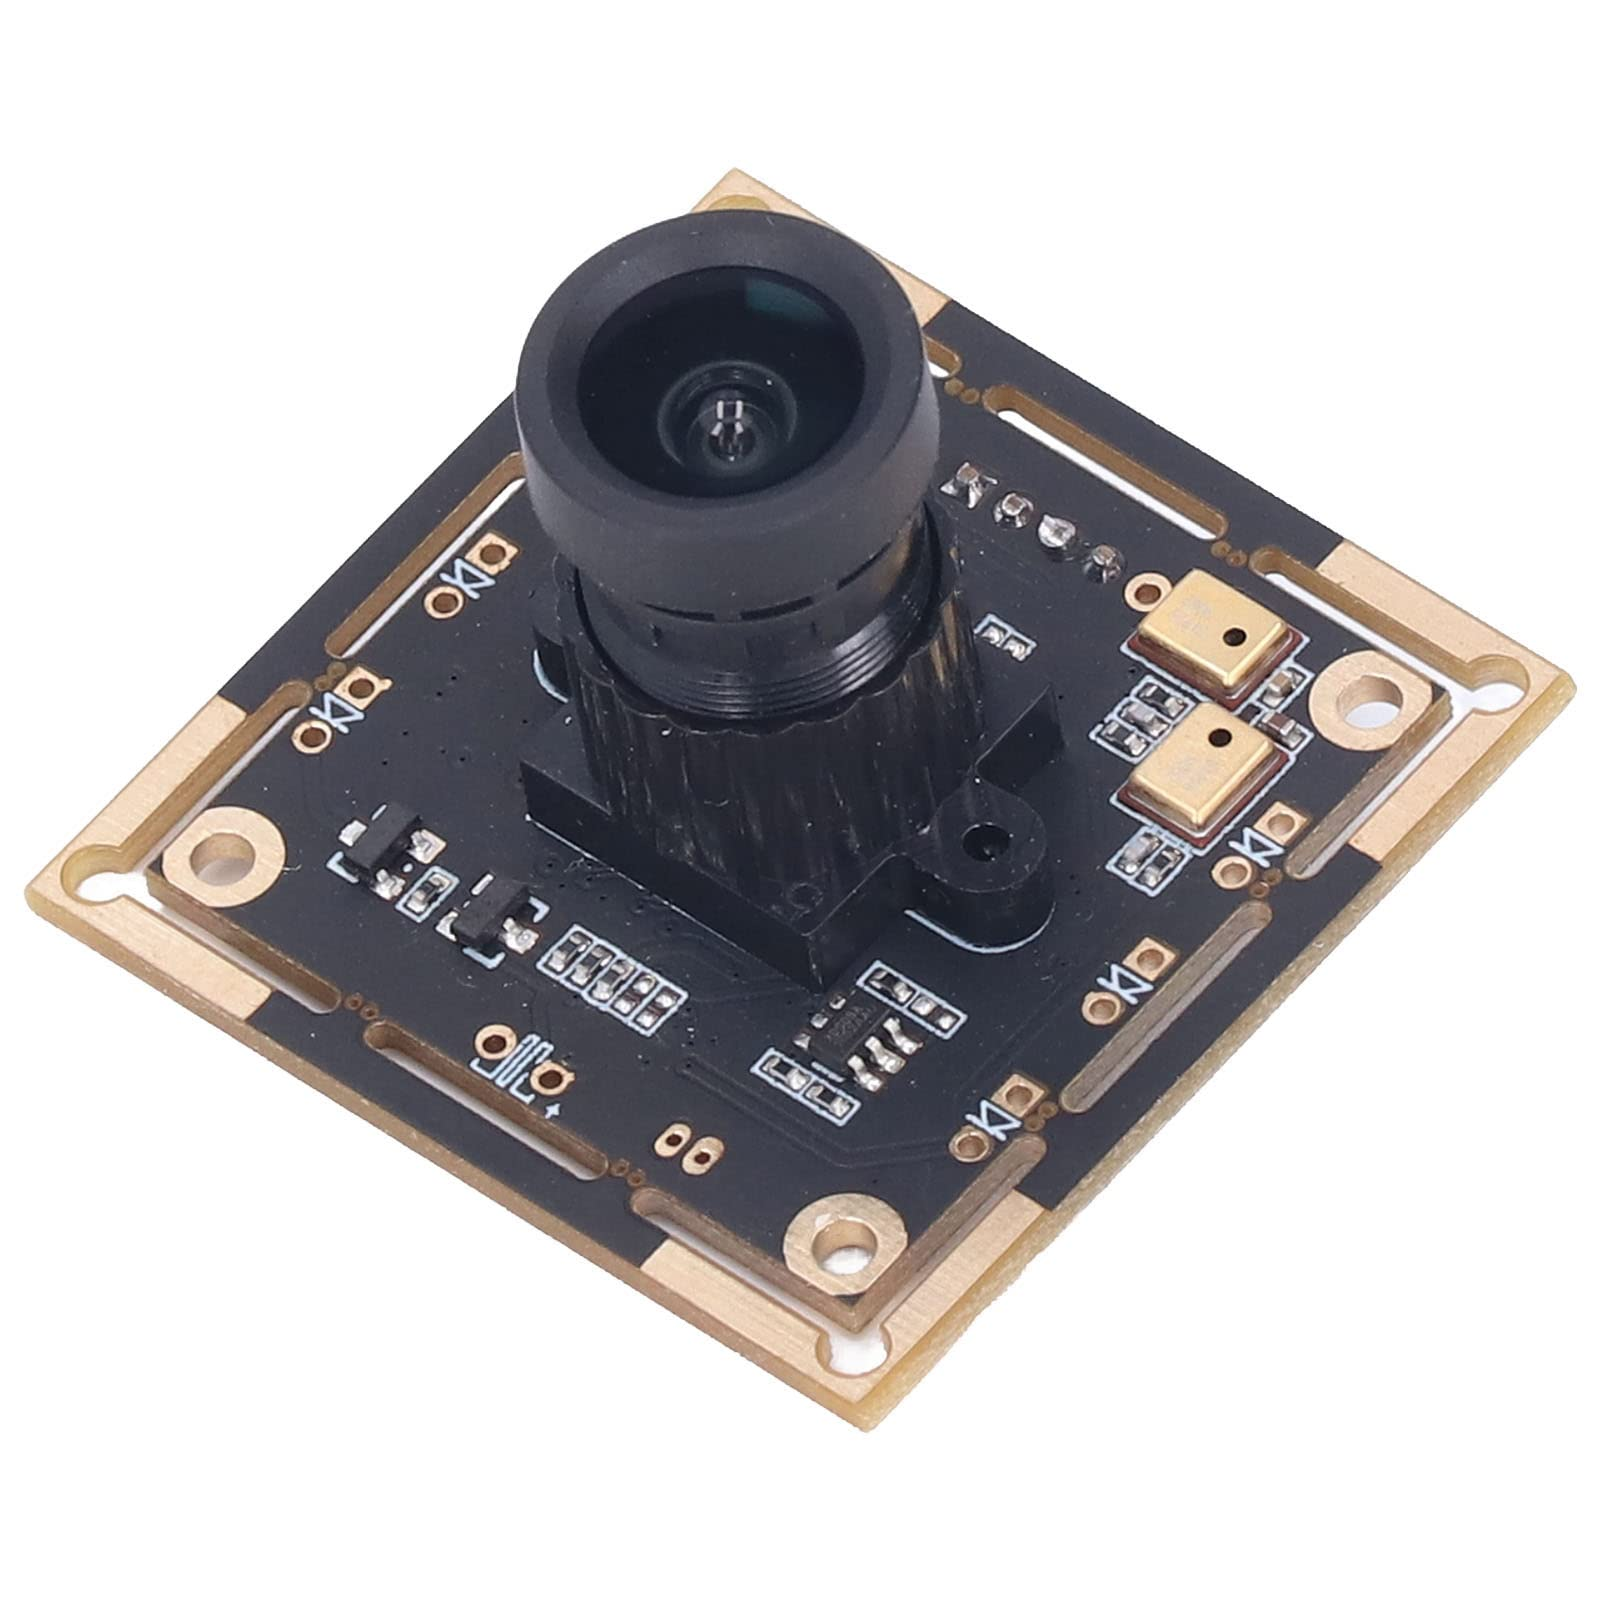
\includegraphics[width=.7\textwidth]{rgbcam}
			\caption{RGB USB camera.}
			\label{fig:rgbcam}
		\end{figure}
	\end{columns}
\end{frame}
\begin{frame}{Vision in robotics}{Sensors characteristics}
	\begin{columns}
		\column{.5\textwidth}
		\begin{block}{}
			\centering
			\textbf{Light might not belong to the visible band of the spectrum.}
		\end{block}

		\column{.5\textwidth}
		\begin{figure}
			\centering
			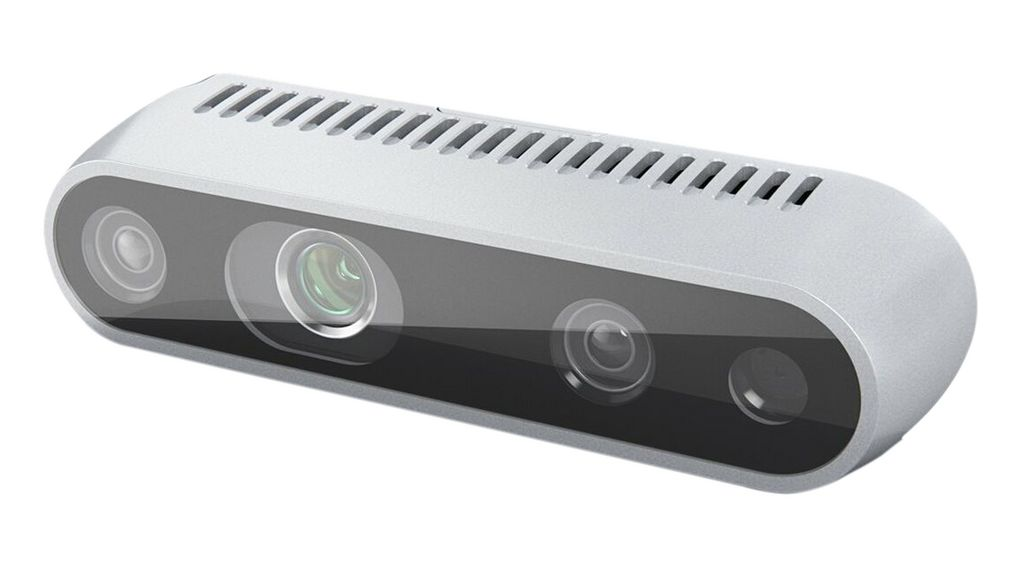
\includegraphics[width=\textwidth]{d435i}
			\caption{Intel RealSense D435i depth camera: RGB and IR sensors.}
			\label{fig:d435i}
		\end{figure}
	\end{columns}
\end{frame}
\begin{frame}{Vision in robotics}{Sensors characteristics}
	\begin{columns}
		\column{.5\textwidth}
		\textbg{Cameras} are usually characterized by:
		\begin{itemize}
			\item \textbg{resolution}, \emph{i.e.}, the number of pixels in the image;
			\item \textbg{field of view}, \emph{i.e.}, the angular extension of the scene (horizontal and vertical);
			\item \textbg{frame rate}, \emph{i.e.}, the number of frames per second;
			\item \textbg{dynamic range}, \emph{i.e.}, the ratio between the maximum and minimum measurable light intensity.
		\end{itemize}

		\column{.5\textwidth}
		\begin{figure}
			\centering
			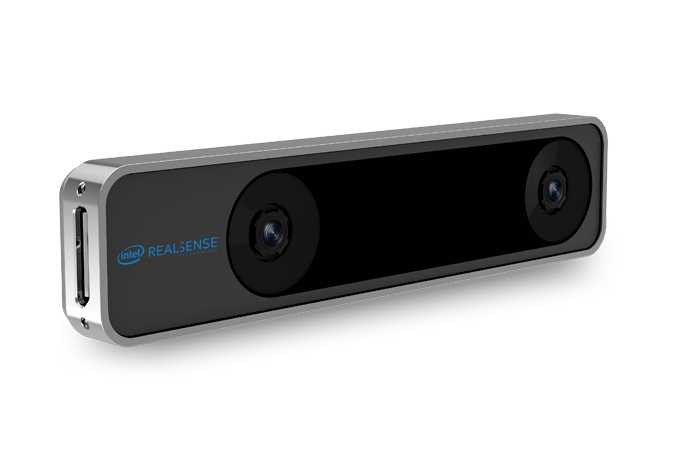
\includegraphics[width=\textwidth]{t265}
			\caption{Intel RealSense T265 tracking camera: two fisheye sensors.}
			\label{fig:t265}
		\end{figure}
	\end{columns}
\end{frame}
\begin{frame}{Vision in robotics}{Sensors characteristics}
	\begin{columns}
		\column{.5\textwidth}
		\begin{block}{}
			\centering
			\textbf{Cameras, and image processing algorithms in general, are usually characterized by a trade-off between resolution and frame rate.}
		\end{block}

		\column{.5\textwidth}
		\begin{figure}
			\centering
			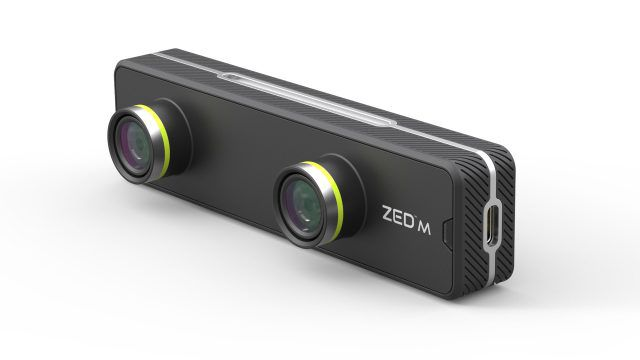
\includegraphics[width=\textwidth]{zedm}
			\caption{ZED Mini stereo tracking camera.}
			\label{fig:zedm}
		\end{figure}
	\end{columns}
\end{frame}
\begin{frame}{Vision in robotics}{Main use cases}
	Visual sensors are usually employed in robotics for:
	\begin{itemize}
		\item \textbg{object detection}, \emph{i.e.}, identifying objects in the scene;
		\item \textbg{object tracking}, \emph{i.e.}, following objects in the scene;
		\item \textbg{localization}, \emph{i.e.}, estimating the robot's position in the environment;
		\item \textbg{mapping}, \emph{i.e.}, building a model of the environment.
	\end{itemize}
	\vspace{.5cm}
	Using the sensor is not enough: \textbg{algorithms} are needed to perform these tasks.\\
	Such algorithms usually run in separate modules.
\end{frame}

% --- Types of frames ---
\begin{frame}{Types of frames}{RGB frame}
	\begin{figure}
		\centering
		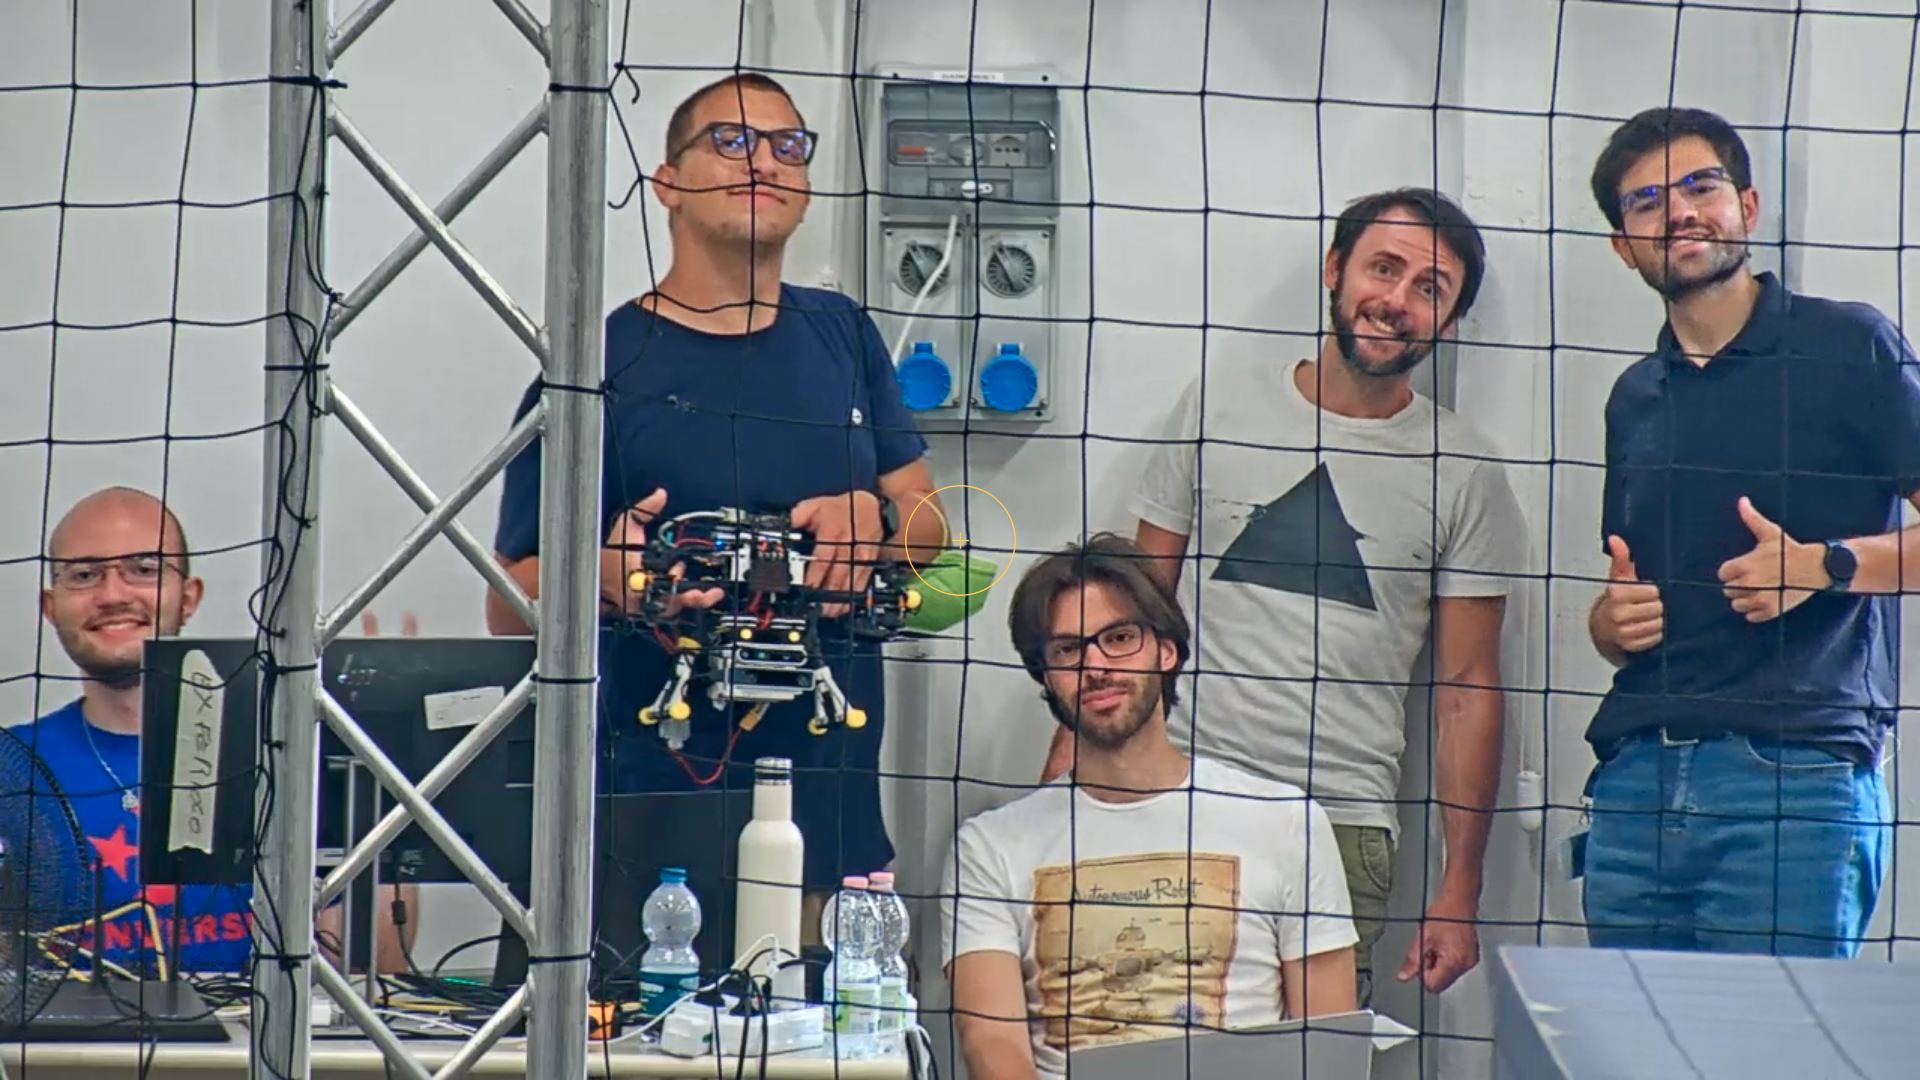
\includegraphics[width=.63\textwidth]{rgb}
		\caption{RGB frame: each pixel contains at least the intensities of the red, green and blue components of the corresponding point in the scene.}
		\label{fig:rgb}
	\end{figure}
\end{frame}
\begin{frame}{Types of frames}{IR frame}
	\begin{figure}
		\centering
		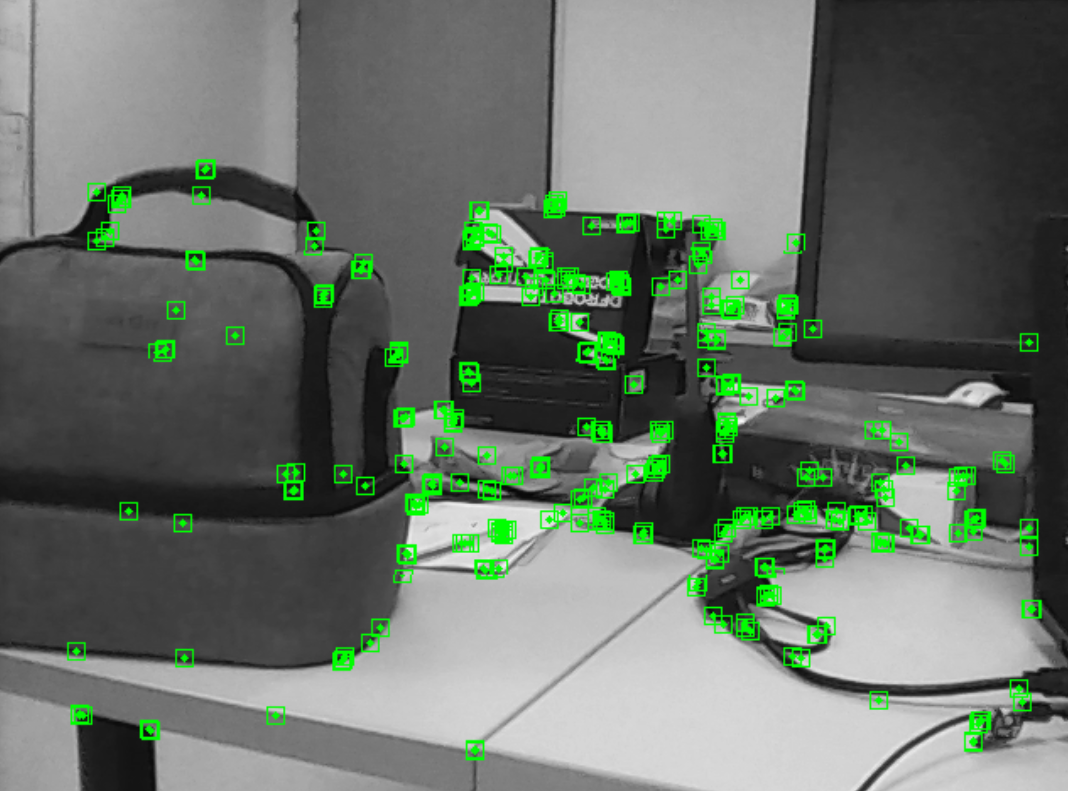
\includegraphics[width=.5\textwidth]{ir}
		\caption{IR frame: each pixel contains the intensity of the corresponding point in the scene.}
		\label{fig:ir}
	\end{figure}
\end{frame}
\begin{frame}{Types of frames}{Depth map frame}
	\begin{figure}
		\centering
		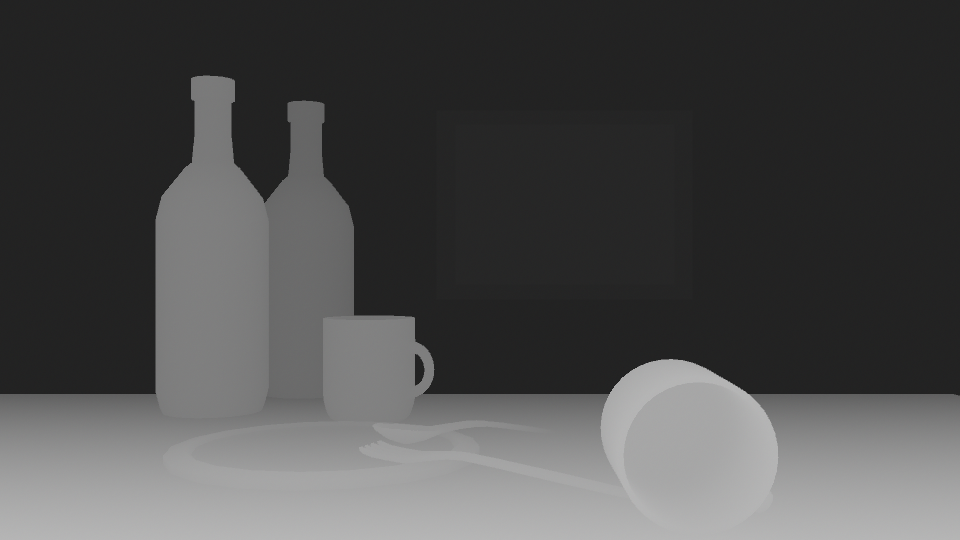
\includegraphics[width=.68\textwidth]{depthmap}
		\caption{Depth map frame: each pixel contains the distance of the corresponding point from the camera.}
		\label{fig:depthmap}
	\end{figure}
\end{frame}

% --- Lens distorsion ---
\begin{frame}{Lens distorsion}{Camera calibration and rectification}
	\begin{columns}
		\column{.5\textwidth}
		\textbg{Pinhole cameras} generally introduce \textbg{radial distorsion} in the images they produce, \emph{i.e.}, \textbg{straight lines appear curved}. This is due to how the light enters the camera through the lens.
		\newline\newline
		A \textbg{camera calibration} procedure is needed to estimate the parameters of the \textbg{distorsion model}, so that a \textbg{rectification map} can then be applied to each frame.

		\column{.5\textwidth}
		\begin{figure}
			\centering
			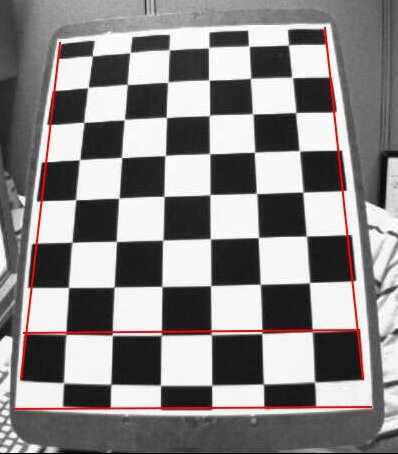
\includegraphics[width=.6\textwidth]{radial}
			\caption{Checkerboard pattern used for camera calibration in the presence of radial distortion.}
			\label{fig:radial}
		\end{figure}
	\end{columns}
\end{frame}
\begin{frame}{Lens distorsion}{Camera calibration and rectification}
	\begin{columns}
		\column{.5\textwidth}
		The calibration procedure usually involves moving a \textbg{checkerboard} of known dimensions in front of the camera, and taking several pictures of it from different angles.
		\newline\newline
		An \textbg{estimation model} can then be used to estimate the parameters of the distorsion model, which can then be used to build the rectification map.

		\column{.5\textwidth}
		\begin{figure}
			\centering
			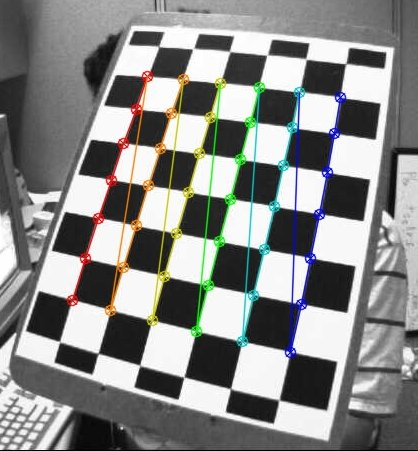
\includegraphics[width=.6\textwidth]{calibration}
			\caption{A frame from a checkerboard calibration procedure.}
			\label{fig:calibration}
		\end{figure}
	\end{columns}
\end{frame}
\begin{frame}{Lens distorsion}{Camera calibration and rectification}
	\begin{columns}
		\column{.5\textwidth}
		The \textbg{rectification map} is a \textbg{lookup table} that associates each pixel in the original frame with a pixel in the rectified frame, \textbg{interpolating} when necessary.
    \newline\newline
    It is usually stored in \textbg{configuration files}, and must be applied to each frame before it can be used by other algorithms.
    \vspace{.45cm}
    \begin{block}{}
      \centering
      \textbf{ROS 2 offers the \href{https://navigation.ros.org/tutorials/docs/camera_calibration.html}{\color{blue}\underline{\texttt{cameracalibrator}}} tool in the \texttt{camera\_calibration} package to perform camera calibration.}
    \end{block}

		\column{.5\textwidth}
		\begin{figure}
			\centering
			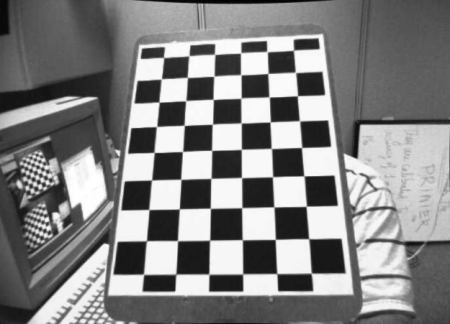
\includegraphics[width=.9\textwidth]{calibrated}
			\caption{Checkerboard pattern after rectification.}
			\label{fig:calibrated}
		\end{figure}
	\end{columns}
\end{frame}


% --- Section 3 ---
% Section 3 - Software tools of the trade
% Roberto Masocco <roberto.masocco@uniroma2.it>
% June 7, 2023

% ### Software tools of the trade ###
\section{Software tools of the trade}
\graphicspath{{figs/section3/}}

% --- OpenCV ---
\begin{frame}{OpenCV}{The de-facto stadard library for computer vision}
	\begin{columns}
		\column{.5\textwidth}
		\only<1>{
			\hspace{-.1cm}\href{https://opencv.org/}{\color{blue}\underline{\textbf{OpenCV}}} is the largest open-source library for real-time \textbg{computer vision} and \textbg{image processing}. It has been developed initially by Intel, and evolved in a \textbg{cross-platform} library supporting \textbg{C++} and \textbg{Python}.
			\newline\newline
			It ships with hundreds of \textbg{APIs} and \textbg{algorithms} to perform a wide variety of image processing and computer vision tasks and computations.
		}
		\only<2>{
			\hspace{-.25cm}In Linux, it is available as \textbg{binary packages}, but the full range of features can be enabled only by \textbg{configuring a source build}.
			\newline\newline
			Its \textbg{elementary data type} is a \textbg{matrix}: \texttt{cv::Mat}.
			\newline\newline
			It is \textbg{heavily optimized} to run on:
			\begin{itemize}
				\item \textbg{parallel CPUs};
				\item \textbg{GPUs} (\emph{e.g.}, \texttt{cv::cuda}, \texttt{cv::ocl});
				\item \textbg{embedded devices} (\emph{e.g.}, Nvidia Jetson).
			\end{itemize}
		}

		\column{.5\textwidth}
		\begin{figure}
			\centering
			
\includegraphics[width=.6\textwidth]{opencv}
			\caption{OpenCV logo.}
			\label{fig:opencv}
		\end{figure}
	\end{columns}
\end{frame}

% --- ROS tools for image processing ---
\begin{frame}{ROS tools for image processing}{A quick overview}
	ROS provides a wide range of tools to acquire, process, and transmit images. The most important ones are:
	\begin{itemize}
		\item \texttt{sensor\_msgs/Image}: the standard ROS message type to transmit images over the DDS layer;
		\item \texttt{sensor\_msgs/CameraInfo}: the standard ROS message type to transmit and parse camera calibration parameters;
		\item \href{https://wiki.ros.org/image_transport}{\color{blue}\underline{\texttt{image\_transport}}}: a ROS package to transmit images over the DDS layer;
		\item \href{https://wiki.ros.org/camera_info_manager}{\color{blue}\underline{\texttt{camera\_info\_manager}}}: a library to parse, use, and store camera calibration parameters from configuration files and messages inside ROS nodes.
	\end{itemize}
\end{frame}
\begin{frame}[fragile]{ROS tools for image processing}{The Image message}
	\begin{columns}
		\column{.9\textwidth}
		\begin{lstlisting}[language=ros2msg, caption=Definition of the \texttt{sensor\_msgs/msg/Image} message.]
std_msgs/Header header

uint32 height
uint32 width

# This can be RGB, BGR, RGBA, BGRA, YUV, Bayer, etc.
string encoding

uint8 is_bigendian
uint32 step
uint8[] data\end{lstlisting}
	\end{columns}
\end{frame}
\begin{frame}{ROS tools for image processing}{Sending images over the DDS}
  Using images and video streams in general over the DDS layer is \textbg{not trivial}, since:
  \begin{enumerate}
    \item we would like some kind of \textbg{specialized transport strategy} to optimize throughput and latency;
    \item the DDS specification is \textbg{not optimized} to transmit \textbg{large} and \textbg{variable-size} data chunks over potentially \textbg{lossy} networks, \emph{e.g.}, WiFi.
  \end{enumerate}
  \texttt{image\_transport} is a ROS 2 library that provides \textbg{wrappers} for \textbg{topic publishers} and \textbg{subscribers}, allowing to transmit images using different \textbg{transports}:
  \begin{itemize}
    \item \texttt{raw}: the default transport, which uses the \texttt{sensor\_msgs/Image} message;
    \item \texttt{compressed}: uses the \texttt{sensor\_msgs/CompressedImage} message, automatically converting frames to \texttt{JPEG} or \texttt{PNG} format;
    \item whatever you want to implement as a \textbg{plugin}.
  \end{itemize}
\end{frame}
\begin{frame}{ROS tools for image processing}{A note on topic statistics}
  \begin{alertblock}{Beware!}
    When measuring image topics publishing rates with \texttt{ros2 topic hz}, especially \textbr{over a lossy network}, you may get \textbr{wrong results}. This is because of:
    \begin{itemize}
      \item the \textbr{Python DDS implementation} not being so efficient;
      \item the \textbr{hz} Python tool buffering messages into a window-based filter.
    \end{itemize}
    To check the real sampling and receiving rates, \textbr{place publishers of ordinary messages} in your code on both ends, and ispect those instead!\\
    Suggestion: \texttt{std\_msgs/Empty}.
  \end{alertblock}
\end{frame}


% --- Section 4 ---
% Section 4 - Composition
% Roberto Masocco <roberto.masocco@uniroma2.it>
% June 7, 2023

% ### Composition ###
\section{Composition}


\end{document}
